\documentclass[11pt]{beamer}
\usetheme{Warsaw}
\usepackage[utf8]{inputenc}
\usepackage{amsmath}
\usepackage{amsfonts}
\usepackage{amssymb}
\usepackage{graphicx}
\usepackage{booktabs}
\usepackage{caption}
\setbeamertemplate{footline}[frame number]
%\setbeamertemplate{caption}[numbered]
\author{Elisa Tirindelli, Guillaume Daudin}
\title{The futility of mercantilist wars. starting from France and Hamburg}
%\setbeamercovered{transparent} 
%\setbeamertemplate{navigation symbols}{} 
\logo{PhD Working Group} 
%\institute{} 
\date{2 September 2016} 
\subject{EHES Conference} 
\begin{document}


\begin{frame}
\titlepage
\end{frame}


\begin{frame}{\textit{European nations were nations of eternal war} (Jefferson, 1823).}
\begin{itemize}
\item{Indeed, from 1700 to 1825, 2 years out of 3 experienced conflict between major European powers.}\\~\\

\item{Rivalry between Great-Britain and France was central (2nd Hundred Years War 1688-1815).}\\~\\

\item{Especially after the death of Louis XIV, mercantile rivalry was an important motivation of Anglo-French wars. (Crouzet 2008, Wallerstein 1980).}\\~\\

\item{Each nation was jealous of the other's commercial success and the British believed war was a good way to curtail them.}
\end{itemize}
\end{frame}


\begin{frame}{\textit{European nations were nations of eternal war} (Jefferson, 1823).}
\begin{itemize}
\item{War of the Polish Succession (1733-1738)}
\item{War of the Austrian Succession (1740(44)–1748)}
\item{Seven Years' War (1756–1763)}
\item{War of American independence (1775(78)–83)}
\item{French Revolutionary Wars (1792–1802)}
\item{Napoleonic Wars (1803–1815)}
\end{itemize}
\end{frame}

\begin{frame}{Total silver trade Fance GB}
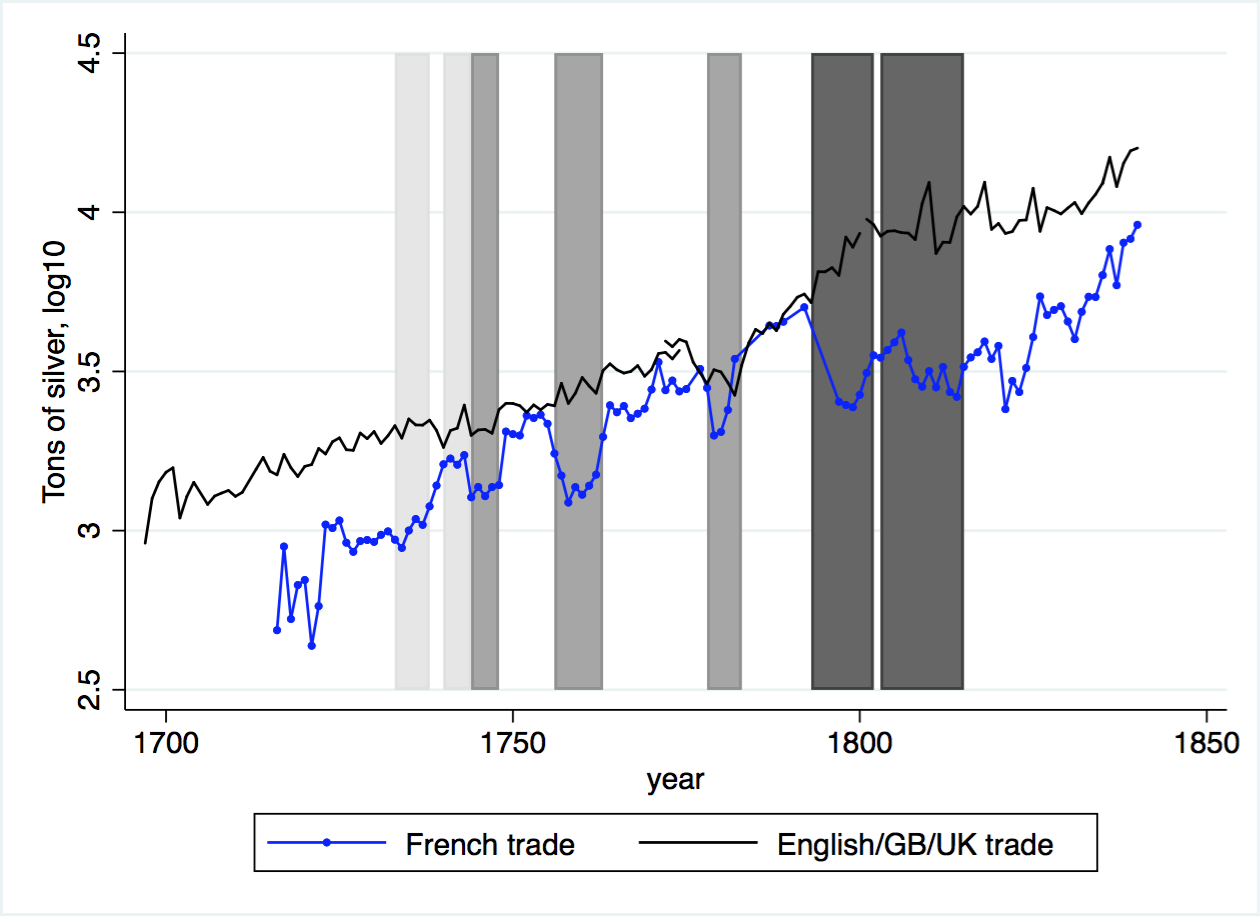
\includegraphics[scale=.5]{Total_silver_trade_FRGB.png}
\end{frame}

\begin{frame}{Research question}
\begin{itemize}
\item{How come the pre-1792 wars did not have a lasting effect on French trade?}\\~\\
\item{Why is it relevant?}
\begin{itemize}
\item{Important to understand the effect of wars in general}
\item{Important to understand (and contrast) the geopolitical history of the 18th and 19th century}
\item{Important to understand the globalization/deglobalization cycle from 1490s to 1840s}
\end{itemize}
\end{itemize}
\end{frame}



\begin{frame}{Literature}
\begin{itemize}
\item{Most of the works are on the 19th and 20th century}\\~\\
\item{No agreement on the exact effect, but most believe there are long-lasting effects of war (Blomberg \& Hess (2004), Glick \& Taylor (2005), but not Barbieri \& Levy (1999)...}\\~\\
\item{The only one of $18^{th}$ century: Rahman (2007)}\\~\\
\item{The resilience of French trade has been remarked by historians (Riley (1984))}
\end{itemize}
\end{frame}


\begin{frame}{Contribution to Literature}
\begin{itemize}
\item{We distinguish trade with neutrals, allies and foes}\\~\\
\item{First study at the sectoral level}\\~\\
\item{Focus on Hamburg, which was neutral during the period (double check)}\\~\\
\item{Conclusion:}
\begin{itemize}
\item{Distinguishing between goods is very important}
\item{War was indeed (very) bad for entrepot trade… but not so much for the rest before the Napoleonic war (Trafalgar? Blockade? Continental system? )}
\end{itemize}
\end{itemize}
\end{frame}

\begin{frame}{Data}
\begin{itemize}
\item{French dataset:}
\begin{itemize}
\item{Data from the \textit{Bureau de la Balance du Commerce}}
\item{3407 bilateral flows between 1713 and 1815}
\item{868 different goods are found in the dataset only 4 of which appear more than 31 times}\\~\\
\end{itemize}
\item{German dataset:}
\begin{itemize}
\item{The data come from the Hamburg import toll register}
\item{1609 observations of aggregate exports flows between 1733 and 1798}
\item{They appear as category of goods, not as single products}
\end{itemize}
\end{itemize}
\end{frame}

\begin{frame}
\begin{center}
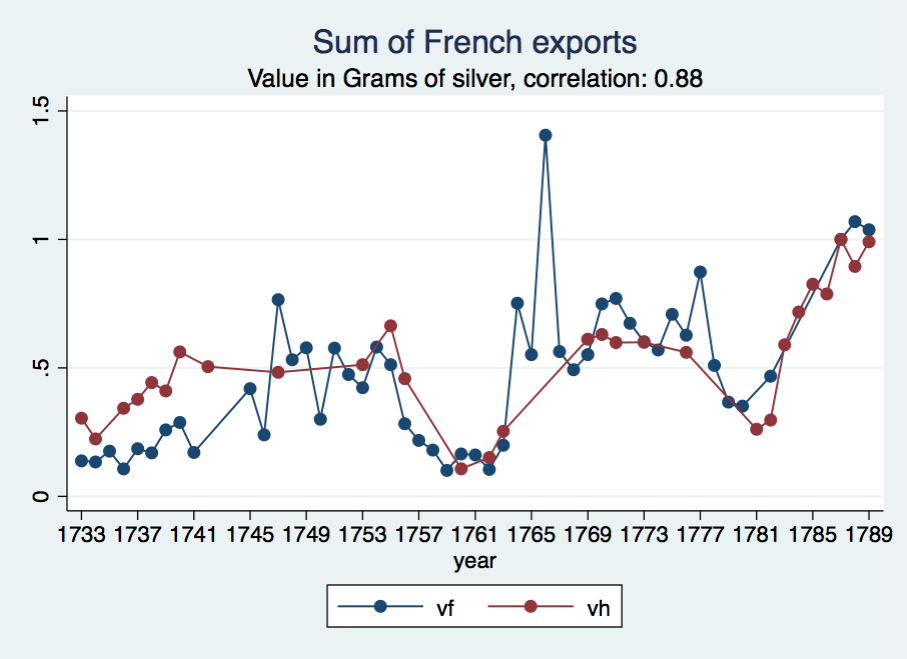
\includegraphics[scale=.3]{long_evolution.png}
\end{center}

\end{frame}

\begin{frame}{Econometric Specification}
\begin{itemize}
\item{I first run a regression on the aggregate exports, distinguishing two wars:
\begin{center}
$\exp(Exports_{i,t})=\beta_0+\beta_1Year+\beta_2War$\\~\\
\end{center} }
\item{I then split exports into  different products:
\begin{center}
$\exp(Exports_{i,t})=\beta_0+\beta_1Year+\beta_2WarCoffee + \beta_3WarEauDeVie+\beta_4WarSugar +\beta_5WarWine +\beta_6WarOther$ \\~\\
\end{center}}
\item{I do so both on Hamburg trade and all French trade.}
\end{itemize}
\end{frame}


%
%\begin{frame}{Impact of wars on Hamburg series (2)}
%\begin{tabular*}{\textwidth}{@{\extracolsep{\fill}}lcccccc}						
%	& \multicolumn{1}{c}{Aggregate} &	\multicolumn{1}{c}{By product} \\
%\cline{2-7}						
%	& \multicolumn{1}{c}{(1)\mbox{\ }} &	\multicolumn{1}{c}{(2)\mbox{\ }}  \\
%\hline		
%All	&-.784 & \\
%&	\raisebox{.7ex}[0pt]{\scriptsize (.110)$^{***}$}  \\				
%Coffee &	 & -.691 &	\\
%&	&\raisebox{.7ex}[0pt]{\scriptsize (.157)$^{***}$} 	\\
%Eau de Vie & &	-.081 	&	\\
%&	&\raisebox{.7ex}[0pt]{\scriptsize (.124)} &	&	\\
%Sugar & &	-.390 	&	\\
%&	&\raisebox{.7ex}[0pt]{\scriptsize (.108)$^{***}$} 	&	&	\\
%Wine & & 	-1.137	&	\\
%&	&\raisebox{.7ex}[0pt]{\scriptsize (.146)$^{***}$} 	&	&	\\
%
%Obs. &	51 &	51 \\
%$ R^2$ &	.883 &		.748  \\
%\hline\hline						
%\end{tabular*}%		
%\end{frame}




\begin{frame}{Impact of wars on Hamburg series (2)}
\begin{tabular*}{\textwidth}{@{\extracolsep{\fill}}lcccccc}						
	& \multicolumn{1}{c}{Aggregate} &	\multicolumn{1}{c}{No breaks} &	\multicolumn{1}{c}{One Break} & \multicolumn{1}{c}{Two Breaks} & \\
\hline					
\hline \\		
All wars &	-0.545 &	 & & & & \\
&	\raisebox{.7ex}[0pt]{\scriptsize (-4.57)$^{***}$} 	& &	& &	& \\				
Coffee &	 & -2.436 & -1.403 &	-1.444  &\\
& &	\raisebox{.7ex}[0pt]{\scriptsize (-5.08)$^{***}$} &	\raisebox{.7ex}[0pt]{\scriptsize (-5.25)$^{***}$} &	\raisebox{.7ex}[0pt]{\scriptsize (-5.20)$^{***}$} &\\
Eau de vie  & &	1.387 &1.387 &	1.387  &\\
& &	\raisebox{.7ex}[0pt]{\scriptsize (4.34)$^{***}$} &	\raisebox{.7ex}[0pt]{\scriptsize (4.34)$^{***}$} &	\raisebox{.7ex}[0pt]{\scriptsize (4.34)$^{***}$} \\
Sugar	& &	-1.874 &-1.874 &	-1.136  \\
& &	\raisebox{.7ex}[0pt]{\scriptsize (-4.25)$^{***}$} &	\raisebox{.7ex}[0pt]{\scriptsize (-4.25)$^{***}$} &	\raisebox{.7ex}[0pt]{\scriptsize (-3.45)$^{***}$} \\
Wine&	 &	0.0711 & 0.0711 &	0.0711 \\
& &	\raisebox{.7ex}[0pt]{\scriptsize (.41)} &	\raisebox{.7ex}[0pt]{\scriptsize (0.41)} &	\raisebox{.7ex}[0pt]{\scriptsize (0.41)} \\
Cons &	6.022 &	-10.14 &	-26.70  &	-111.3 \\
&	\raisebox{.7ex}[0pt]{\scriptsize (1.56)} &	\raisebox{.7ex}[0pt]{\scriptsize (-0.59)} &	\raisebox{.7ex}[0pt]{\scriptsize (-1.61)} &	\raisebox{.7ex}[0pt]{\scriptsize (-7.55)} \\
\hline 
Obs &	76 &	347 &	347  & 347 \\
$ R^2$ &	.319 &	.460 &	.556  & .645 \\

\hline\hline						
\end{tabular*}%
\end{frame}

\begin{frame}{Impact of wars on Hamburg series (3)}
\begin{center}
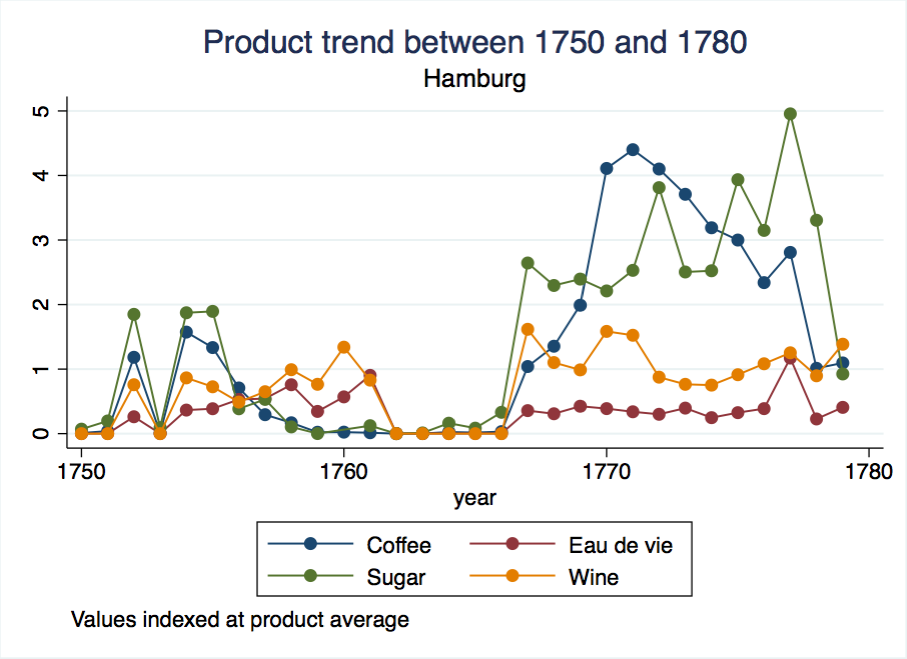
\includegraphics[scale=.3]{hamburg_product_1780.png}
\end{center}
\end{frame}

\begin{frame}{Impact of wars on Hamburg series (4)}
\begin{center}
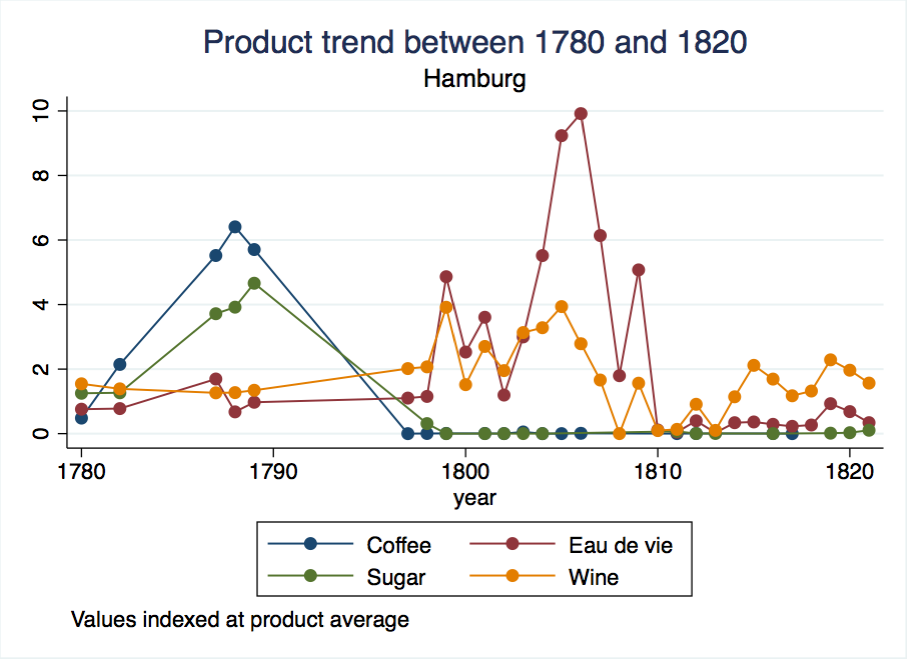
\includegraphics[scale=.3]{hamburg_product_1820.png}
\end{center}
\end{frame}

%\begin{frame}{Impact of wars on all neutral trading partners (1)}
%\begin{itemize}
%\item{I first run a regression on the aggregate exports:
%\begin{center}
%$\exp(Exports_{i,t})=\beta_0+\beta_1Year+\beta_2Adversaries+ \beta_3Allies+ \beta_4Neutral+ \sum_{i}\gamma_iCountry_i+\sum_{i}\delta_iCountry_iYear$\\~\\
%\end{center} }
%\item{I then split exports into  different products:
%\begin{center}
%$\exp(Exports_{i,t})=\alpha+ \sum_{i}\beta_{i}Product_iNeutral +\sum_i \gamma_iProduct_iAllies +\sum_i\delta_iProduct_iAdversaries + \sum_{ij}\lambda_iCountry_iProduct_j+\sum_{i}\theta_iCountry_iYear+ \sum_{i}\phi_iProduct_iYear$
%\end{center}}
%\end{itemize}
%\end{frame}

\begin{frame}{Impact of wars on all neutral trading partners }
\begin{tabular*}{\textwidth}{@{\extracolsep{\fill}}lcccccc}						
	& \multicolumn{1}{c}{Aggregate} &	\multicolumn{1}{c}{No breaks} &	\multicolumn{1}{c}{One Break} & \multicolumn{1}{c}{Two Breaks} & \\
\hline					
\hline \\		
All wars &	-0.373 &	 & & & & \\
&	\raisebox{.7ex}[0pt]{\scriptsize (-3.92)$^{***}$} 	& &	& &	& \\				
Coffee &	 & -1.991 & -1.188 &	-1.188  &\\
& &	\raisebox{.7ex}[0pt]{\scriptsize (-6.67)$^{***}$} &	\raisebox{.7ex}[0pt]{\scriptsize (-7.32)$^{***}$} &	\raisebox{.7ex}[0pt]{\scriptsize (-7.32)$^{***}$} &\\
Eau de vie  & &	0.953 &0.952 &	0.953  &\\
& &	\raisebox{.7ex}[0pt]{\scriptsize (5.50)$^{***}$} &	\raisebox{.7ex}[0pt]{\scriptsize (5.50)$^{***}$} &	\raisebox{.7ex}[0pt]{\scriptsize (5.50)$^{***}$} \\
Sugar	& &	-1.657 &-1.656 &	-1.066  \\
& &	\raisebox{.7ex}[0pt]{\scriptsize (-6.12)$^{***}$} &	\raisebox{.7ex}[0pt]{\scriptsize (-6.12)$^{***}$} &	\raisebox{.7ex}[0pt]{\scriptsize (-5.12)$^{***}$} \\
Wine&	 &	0.061 & 0.061 &	0.062 \\
& &	\raisebox{.7ex}[0pt]{\scriptsize (0.49)} &	\raisebox{.7ex}[0pt]{\scriptsize (0.49)} &	\raisebox{.7ex}[0pt]{\scriptsize (0.50)} \\
Cons &	-40.993 &	-23.09 &	109.7  &	278.7 \\
&	\raisebox{.7ex}[0pt]{\scriptsize (-7.19)$^{***}$} &	\raisebox{.7ex}[0pt]{\scriptsize (-2.01)$^{*}$} &	\raisebox{.7ex}[0pt]{\scriptsize (1.94)} &	\raisebox{.7ex}[0pt]{\scriptsize (3.03)$^{**}$} \\
\hline 
Obs &	789 &	3145 &	3145  & 3145 \\
$ R^2$ &	.623 &	.787 &	.800  & .815 \\

\hline\hline						
\end{tabular*}%
\end{frame}

\begin{frame}{Impact of wars on all neutral trading partners (3)}
\begin{center}
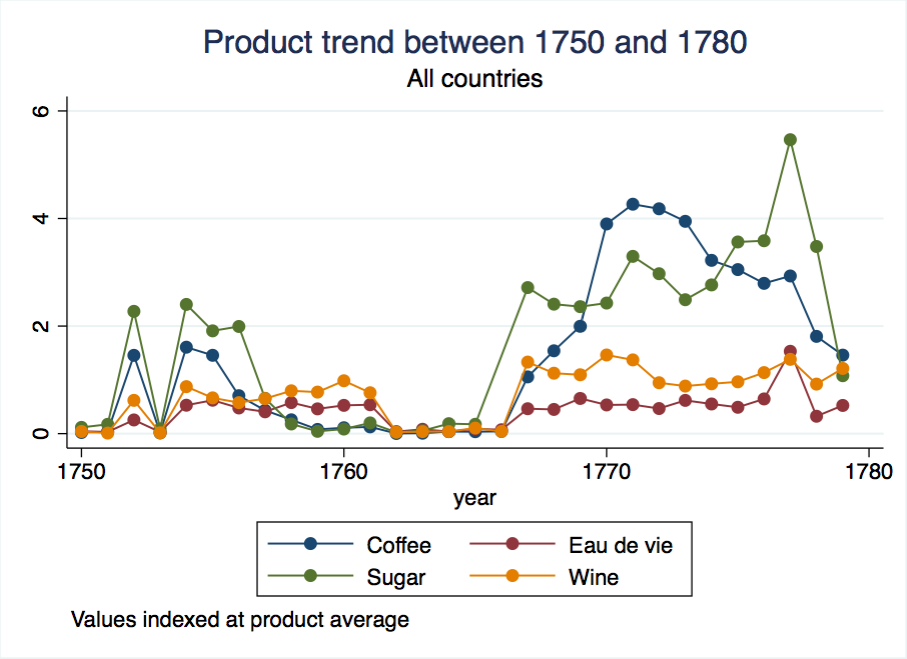
\includegraphics[scale=.3]{allcountry_product_1780.png}
\end{center}
\end{frame}

\begin{frame}{Impact of wars on all neutral trading partners (4)}
\begin{center}
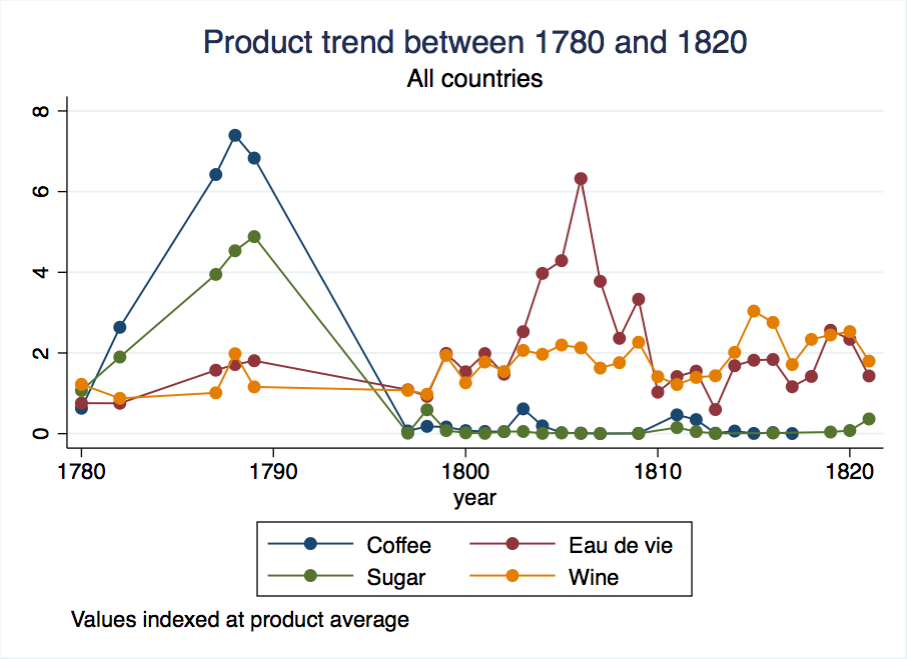
\includegraphics[scale=.3]{allcountry_product_1820.png}
\end{center}
\end{frame}

\begin{frame}{Impact of Continental blockade vs Mercantilist War}
\begin{tabular*}{\textwidth}{@{\extracolsep{\fill}}lcccccc}						
 &	\multicolumn{1}{c}{No breaks} &	\multicolumn{1}{c}{One Break} & \multicolumn{1}{c}{Two Breaks} & \\
\hline					
\hline \\					
Mercantilist War Foes & -2.811 & -1.347 &	-1.348  &\\
&	\raisebox{.7ex}[0pt]{\scriptsize (-6.08)$^{***}$} &	\raisebox{.7ex}[0pt]{\scriptsize (-2.96)$^{***}$} &	\raisebox{.7ex}[0pt]{\scriptsize (-2.96)$^{***}$} &\\
R\&N War Foes &	0.098 &0.098 &	0.098  &\\
 &	\raisebox{.7ex}[0pt]{\scriptsize (0.44)} &	\raisebox{.7ex}[0pt]{\scriptsize (0.44)} &	\raisebox{.7ex}[0pt]{\scriptsize (0.44)} \\
Mercantilist War Neutral &	-2.572 &2.577 &	-1.238  \\
 &	\raisebox{.7ex}[0pt]{\scriptsize (-5.69)$^{***}$} &	\raisebox{.7ex}[0pt]{\scriptsize (-5.71)$^{***}$} &	\raisebox{.7ex}[0pt]{\scriptsize (-2.99)$^{***}$} \\
R\&N War Neutral	 &	0.074 & 0.074 &	0.075 \\
 &	\raisebox{.7ex}[0pt]{\scriptsize (0.59)} &	\raisebox{.7ex}[0pt]{\scriptsize (0.59)} &	\raisebox{.7ex}[0pt]{\scriptsize (0.60)} \\
Cons &	-23.09 &	109.7  &	278.7 \\
 &	\raisebox{.7ex}[0pt]{\scriptsize (-2.01)$^{*}$} &	\raisebox{.7ex}[0pt]{\scriptsize (1.94)} &	\raisebox{.7ex}[0pt]{\scriptsize (3.03)$^{**}$} \\
\hline 
Obs  &	3145 &	3145  & 3145 \\
$ R^2$  &	.787 &	.800  & .815 \\

\hline\hline						
\end{tabular*}%
\end{frame}




\begin{frame}{Conclusion}
\begin{itemize}
\item{We have known for some time that French trade was resilient to war.}
\begin{itemize}
\item{Use of the neutral flag.}
\item{Re-routing of exports.}
\end{itemize}~\\
\item{This was becoming more and more difficult, as the treatment of neutrals was becoming stricter and stricter.}\\~\\
\item{What other questions?}
\begin{itemize}
\item{When was the turning point? The 1790s or the 1800 (and the Continental System and the Blockade).}
\item{Probably not the loss of colonies by itself.}
\item{Maybe the loss of positive effects for some goods?}\\~\\
\end{itemize}
\item{All in all, the trading system seems to have been quite resilient.}

\end{itemize}
\end{frame}




%\begin{frame}{Next steps: (2)}
%\begin{itemize}
%
%\item{Cluster countries by trade composition:}
%\begin{itemize}
%\item{K-clustering}
%\item{Correlation of total trade by product}\\~\\
%\end{itemize}
%\item{Look at war by war case. }\\~\\
%\item{Robustness checks and existence of of maximum in poisson regression.}\\~\\

%\end{itemize}
%\end{frame}

\begin{frame}
\begin{center}
\Huge{Thank you!}
\end{center}

\end{frame}


\end{document}

